\documentclass{article}
% --- watermark (auto-inserted) ---
\usepackage{xcolor}
\usepackage{xfp}% \fpeval; in the kernel since 2022, harmless on older LaTeX
\usepackage{draftwatermark}
\newlength{\watermarkTextWidth}
\AddToHook{begindocument/end}{%
  \SetWatermarkText{\normalfont Generated by The Agentic Scientist}%
  \SetWatermarkFontSize{10pt}%
  \SetWatermarkLightness{0.85}%
  \settowidth{\watermarkTextWidth}{\normalfont\fontsize{10pt}{12pt}\selectfont Generated by The Agentic Scientist}%
  \edef\watermarkScale{\fpeval{0.8 * sqrt(\paperwidth**2 + \paperheight**2) / \watermarkTextWidth}}%
  \edef\watermarkAngle{\fpeval{atand(\paperheight/\paperwidth)}}%
  \SetWatermarkScale{\watermarkScale}%
  \SetWatermarkAngle{\watermarkAngle}%
}
% --- end watermark ---
\usepackage{iclr2026_conference,times}
\usepackage{amsmath,amssymb,booktabs,graphicx,subcaption,longtable}
\usepackage{hyperref,url}
\newcommand{\E}{\mathbb{E}}
\newcommand{\Var}{\operatorname{Var}}
\newcommand{\clip}{\operatorname{clip}}
\title{Frozen-Score Controls for Mean Inference:\\Width Gains and Coverage Limitations}
\author{}

\begin{document}
\maketitle

\begin{abstract}
Can confidence intervals become narrower when labels, unlabeled observations, and the predictor are unchanged? We examine inference-side calibration of frozen scores for a binary population mean, using paired interval records from seven evaluation conditions and 256 repetitions per condition. The associated implementation fits honest, regularized score controls and returns a stabilized asymptotic interval; its bounded finite-sample construction is separate and unmeasured. Relative to the evaluated PPI++ comparator, mean width decreases in only one condition, by 0.000302, and increases in the other six. In the condition with population mean 0.0068, PPI++ coverage is 0.551 and 115 intervals collapse, whereas score-control coverage is 0.930 without collapse. However, the score-control width difference from exact-binomial inference is inconclusive, and pooled empirical coverage of 0.943 does not establish nominal validity. These results support condition-specific comparisons, not uniformly shorter valid intervals. Missing condition generators, sample-size metadata, and a matched calibration ablation limit reproducibility and mechanistic attribution.
% @evidence[[paper_data.json#/final_evaluation]]
% @evidence[[analysis_results.json#/cases]]
% @evidence[[source_evidence/calibration/program.py#L123-L192]]
\end{abstract}

\section{Introduction}
Scientific inference increasingly uses a small collection of expensive gold-standard labels together with predictions available on a larger collection of observations. The scientific target is often simpler than individual prediction: a prevalence, an average response, or another population summary. Prediction-powered inference uses labels to correct prediction error rather than treating machine predictions as truth \citep{Angelopoulos2023PPI}. This distinction matters when the predictor is useful but imperfect. It also motivates a constrained question: once the observations and predictor are fixed, is there still room to improve the uncertainty attached to the population mean?

The constraint excludes acquiring labels, enlarging the unlabeled sample, or replacing the prediction model. It does not exclude fitting an inference-side transformation of its scalar output. A nonlinear transformation might make the score a better control variate for the outcome. Yet estimating this transformation consumes statistical information, and an interval can become shorter simply because its uncertainty calculation is inadequate. Thus, width alone cannot answer the question. Any efficiency claim must distinguish information extraction from estimation noise and must confront repeated-sampling coverage.

We study \emph{honest frozen-score controls}: complementary labeled subsets fit a small regularized calibration family, while held-out labels correct its errors. A fixed-control variance identity explains the potential benefit of approximating the conditional outcome mean given the score. It also identifies a boundary on what calibration can accomplish: it cannot recover information absent from the frozen score. The evaluated interval uses a stabilized asymptotic variance approximation. A distinct bounded construction clarifies what a finite-sample argument would require, but its empirical efficiency is not observed here.

Our central empirical finding is limited and asymmetric. Among seven conditions, only C2 has a negative paired mean-width difference relative to the evaluated PPI++ interval; the remaining six differences are positive. A low-prevalence condition exposes severe undercoverage and collapsed intervals for two asymptotic comparators. The score-control interval avoids these observed collapses but does not establish nominal coverage or an advantage over exact inference. These are comparisons of recorded intervals, not a causal test of nonlinear calibration.
% @evidence[[paper_data.json#/final_evaluation/evaluation_evidence/episodes/0/solution/case_summaries]]

The contributions are threefold: separating fixed-score efficiency potential from inference assumptions; a complete paired comparison retaining favorable and unfavorable conditions; and a failure analysis distinguishing non-collapse, narrowness, and validity. Missing generators and controlled ablations remain explicit limitations rather than being filled with inferred mechanisms.

\begin{figure}[t]
\centering
\begin{minipage}[c][1.8in][c]{\textwidth}
\centering

\includegraphics[width=\textwidth,height=1.8in,keepaspectratio]{figures/frozen_score_overview.png}
\end{minipage}
\caption{Inference with unchanged observations and a frozen predictor. Complementary labeled folds fit score-only controls; held-out residual correction targets the population mean. The evaluated stabilized asymptotic interval and the separate, unmeasured bounded safety construction must not be conflated. No new labels or predictor training are part of this comparison.}
\label{fig:overview}
% @evidence[[source_evidence/calibration/program.py#L123-L192]]
\end{figure}

\section{Related Work}
\paragraph{Prediction-assisted estimation.}
PPI supplies the central correction principle: combine predictions with a labeled estimate of their error \citep{Angelopoulos2023PPI}. PPI++ adapts the contribution of predictions to improve statistical and computational efficiency under its assumptions \citep{Angelopoulos2023PPIpp}. Our empirical baseline is the \emph{evaluated PPI++ comparator}, not a claim about every implementation or theoretical formulation of PPI++. Classical control variates likewise exploit correlated auxiliary quantities to reduce Monte Carlo variance \citep{Glasserman2004}. Survey calibration and model-assisted estimation use auxiliary information in a related spirit \citep{DevilleSarndal1992,Sarndal1992}; their finite-population targets should not be silently substituted for the superpopulation target studied here. Missing-data theory provides additional context for assumptions connecting observed and unobserved outcomes \citep{LittleRubin2019}.

\paragraph{Fitted controls and sample separation.}
Residualization with estimated functions is familiar in semiparametric inference \citep{Robinson1988,VanDerVaart1998}. Double/debiased machine learning combines orthogonal corrections with sample separation to control nuisance-estimation effects \citep{Chernozhukov2018DML}. We use complementary training folds, but do not infer finite-sample validity from that structural similarity. Ridge regularization \citep{HoerlKennard1970}, generalized cross-validation \citep{Golub1979GCV}, and cross-validatory prediction assessment \citep{Stone1974} motivate the archived calibration choices. A small linear-spline dictionary is a standard approximation device \citep{Hastie2009}, not evidence that the dictionary matches the unknown conditional mean in these conditions.

\paragraph{Intervals near the boundary.}
Exact binomial inversion \citep{BlythStill1983}, score-based intervals \citep{Newcombe1998}, adjusted approximations \citep{AgrestiCoull1998}, and analyses of erratic Wald coverage \citep{BrownCaiDasGupta2001} motivate retaining an exact reference rather than comparing only against a normal approximation. A Wilson-style adjustment to a fitted-control estimator is not the binomial Wilson procedure. For bounded observations, concentration inequalities \citep{Hoeffding1963} and empirical-Bernstein bounds \citep{MaurerPontil2009} offer another route, at potentially substantial width cost. Variance-sensitive concentration also appears in sequential allocation \citep{Audibert2009}; no active allocation is used here. The relevant distinction is between an assumption-dependent coverage argument and an observed coverage estimate, not between a favorable and unfavorable average width.

\section{Method}
\subsection{Target, Constraints, and the Efficiency Question}
Let $(Y_i,S_i)_{i=1}^n$ denote labeled observations, where $Y_i\in\{0,1\}$ and $S_i=f(X_i)\in[0,1]$. The unlabeled observations contribute scores $(S_j^U)_{j=1}^N$. The predictor $f$ is fixed. The target is
\begin{equation}
\mu=\E[Y],\qquad
\Pr\{\mu\in I\}\geq 1-\alpha,
\label{eq:target}
\end{equation}
with interval width $|I|$ as the efficiency criterion. The nominal level in the recorded interface is $1-\alpha=0.95$. The method receives only labeled outcomes and labeled/unlabeled scores, not a population truth or condition identity.
% @evidence[[source_evidence/calibration/program.py#L1-L44]]

For the analysis of estimators, assume independent iid labeled pairs and iid unlabeled scores from the same population, with the predictor frozen independently of the inference labels. These are explicit statistical assumptions, not facts established by the unidentified condition generators. ``Fixed inputs'' means that compared methods have the same observations within a repetition. It does not mean conditioning away all repeated-sampling randomness, nor does it change the target to the realized mean of an observed finite pool. Different targets require different coverage arguments.

The practical question is whether a fitted transformation of $S$ can reduce width \emph{without losing the coverage requirement}. We do not optimize the reported width over the observed repetitions. Instead, we compare the sealed interval outputs and retain coverage and width as separate outcomes. This prevents interpreting a narrow but under-covering interval as an efficiency solution.

\subsection{Design Rationale: What a Frozen Score Can Offer}
For a fixed square-integrable control $g$, write $\rho=N/(n+N)$ and consider
\begin{equation}
\widehat\mu_g=\overline{Y-\rho g(S)}_L+\rho\overline{g(S)}_U,
\quad
\Var(\widehat\mu_g)=\frac{\Var(Y-\rho g(S))}{n}
+\frac{\rho^2\Var(g(S))}{N}.
\label{eq:fixed}
\end{equation}
Equal score distributions in the labeled and unlabeled samples ensure cancellation of the control's expectation. There is no requirement that $g$ itself predict the outcome without bias. The finite-$N$ factor recognizes uncertainty in the unlabeled average rather than treating it as a known population moment.

Let $m(S)=\E[Y\mid S]$. Expanding the variance in Equation~\ref{eq:fixed} gives
\begin{align}
\Var(\widehat\mu_m)&=\frac{\E[\Var(Y\mid S)]}{n}
+\frac{\Var(m(S))}{n+N},\label{eq:oracle}\\
\Var(\widehat\mu_g)-\Var(\widehat\mu_m)
&=\frac{\rho}{n}\Var\{g(S)-m(S)\}.\label{eq:excess}
\end{align}
% @evidence[[source_evidence/calibration/METHOD.md#Oracle-frontier-and-asymptotic-qualifications]]
The identity describes a population oracle among fixed controls, up to additive constants. It suggests a rationale for nonlinear calibration when the score--outcome relationship departs from an affine function. It is not a claim that the finite fitted dictionary attains this oracle. Nor is a variance identity automatically a confidence-interval theorem for a data-adaptive control. Constant or uninformative scores offer no auxiliary variance reduction in this calculation; labels still determine the irreducible outcome-noise term.

\subsection{Archived Honest Calibration Construction}
The inspectable implementation associated with the selected method uses two labeled folds and two unlabeled folds from independent permutations initialized by the repetition seed. For labeled fold $L_k$, the opposite labeled fold fits $g_{-k}$. Its intercept, feature centering, feature scaling, spline knots, and regularization choice all use that training fold only. Neither held-out scores nor unlabeled scores tune the calibration. After fitting, evaluated controls are clipped to $[0,1]$.
% @evidence[[source_evidence/calibration/program.py#L51-L102]]
% @evidence[[source_evidence/calibration/program.py#L123-L171]]

The family includes an intercept, a ridge affine function, and linear splines with training-score quantile knots. Up to three quartile knots become available at training size 16; up to seven quantile knots become available at size 64. The ridge penalties are $\{0.001,0.01,0.1,1,10\}$. Training-only GCV chooses a fit relative to the constant candidate. Constant-score or very small training samples retain the intercept. These choices specify the archived code, not measured hyperparameter sensitivities.
% @evidence[[source_evidence/calibration/program.py#L58-L93]]

The fold estimate and aggregate estimate are
\begin{equation}
\widehat\mu_k=\overline{Y-\rho g_{-k}(S)}_{L_k}
+\rho\overline{g_{-k}(S)}_{U_k},\qquad
\widehat\mu=\sum_{k=1}^{2}w_k\widehat\mu_k,\quad w_k=|L_k|/n.
\label{eq:fold}
\end{equation}
% @evidence[[source_evidence/calibration/program.py#L135-L172]]
Training separation prevents an observation's label from fitting its own control. It does not make the fitted folds unconditionally independent: a label held out in one fold trains the other fold's control. The implementation retains all held-out residuals and unlabeled control values for a pooled variance approximation. It also contains an affine-only matched function, but no measured affine-versus-spline ablation is available. Therefore, the empirical comparison concerns the complete interval construction.

\subsection{Returned Interval and Separate Safety Construction}
Let $R_i=Y_i-\rho g_{-k(i)}(S_i)$ and $Q_j=\rho g_{-k(j)}(S_j^U)$. The archived asymptotic calculation is
\begin{equation}
\widehat V=\frac{s_R^2}{n}+\frac{s_Q^2}{N},\quad
a=\frac{z_{1-\alpha/2}^2}{n},\quad
c=\frac{\widehat\mu+a/2}{1+a},\quad
r=\frac{z_{1-\alpha/2}\sqrt{\widehat V+z_{1-\alpha/2}^2/(4n^2)}}{1+a}.
\label{eq:stabilized}
\end{equation}
The endpoints are $\clip(c-r,0,1)$ and $\clip(c+r,0,1)$. This boundary stabilization supplies a positive radius when the empirical variance vanishes, but it does not prove coverage for a fitted-control estimator. The pooled variance also approximates unequal fold weights when sample sizes are odd. For $n<16$, a sample-size-only rule instead returns a labeled-only Clopper--Pearson interval. This branch does not confer exact validity on the other sample sizes.
% @evidence[[source_evidence/calibration/program.py#L172-L185]]
% @evidence[[source_evidence/calibration/program.py#L246-L259]]

The same source computes a distinct empirical-Bernstein interval by bounding each held-out residual mean and unlabeled control mean. Conditional on training, their ranges are $[-\rho,1]$ and $[0,\rho]$. Componentwise bounds, a union bound, and the same fixed nonnegative fold weights give a finite-sample argument under the iid assumptions. Crucially, these endpoints are not returned by the primary interface, compared with the asymptotic endpoints, or selected by their widths. No coverage or width measurement for that safety construction is available. Supplementary Information supplies its argument and the fixed-control variance derivation.
% @evidence[[source_evidence/calibration/program.py#L109-L185]]

\section{Experimental Protocol and Evidence Scope}
\subsection{Paired Records and Comparators}
The completed sealed evaluation contains 256 seeded repetitions, with seven conditions in each repetition. We denote the conditions C1--C7, preserving their recorded identities. Every record supplies the truth, the score-control endpoints, and endpoints for evaluated PPI++, PPI, labeled-only asymptotic mean inference, labeled-only exact-binomial inference, and a full-range sanity interval. The inferential tables include all five nontrivial methods; $[0,1]$ is retained as a sanity reference rather than an efficiency headline. No scored repetition or unfavorable condition is removed.
% @evidence[[paper_data.json#/final_evaluation/evaluation_evidence/episodes]]

The records omit condition generators, dataset names, per-condition $n,N$, raw scores, and label arrays. Recorded truths do not identify calibration nonlinearity, distribution shift, or predictor quality. All conditions are included, but no separately named transfer task is evidenced. These are evaluation-condition comparisons, not established cross-domain generalization.

Comparator versions and internal fitting details are unavailable; conclusions apply to the supplied endpoints. The archived calibration source and entrypoint are readable, but a separate final source tree is unavailable for file-by-file identity verification. Source-level method descriptions are therefore distinguished from sealed numerical results: neither a hash nor method-family alignment proves exact implementation identity.

\subsection{Uncertainty and Reporting Rules}
For each condition and method, we recompute width as upper minus lower and coverage as inclusion of the recorded truth in the closed interval. Coverage uncertainty is a pointwise equal-tailed exact-binomial interval for the repetition count. For a comparator $b$, define the paired difference
\begin{equation}
D_r=|I_{\mathrm{control},r}|-|I_{b,r}|,\qquad
\overline D\ \pm\ t_{0.975,R-1}\,s_D/\sqrt R.
\label{eq:paired}
\end{equation}
Here $R$ is the number of repetitions. Negative differences mean narrower recorded intervals, not better coverage. The paired-$t$ interval summarizes mean differences; unlike exact-binomial coverage limits, it is approximate \citep{Student1908}. The calculations reproduce the supplied condition summaries to numerical precision and use their endpoint records rather than repeatedly counting summaries attached only to the initial record.
% @evidence[[scripts/build_artifacts.py]]
% @evidence[[paper_data.json#/final_evaluation/evaluation_evidence/episodes/0/solution/case_summaries]]

These intervals assume a repeated-sampling interpretation that distinct seeds alone do not verify. They are pointwise, not simultaneous. Multiplicity changes the question \citep{BenjaminiHochberg1995}; no multiple-testing procedure or familywise gain claim is made. All comparisons are retained regardless of sign. Conditions within a seed may share randomness, so pooled coverage is descriptive, not a binomial estimate from independent condition--repetition pairs.

The sealed evaluation is recorded as completed and qualified. That procedural outcome does not certify exact nominal coverage, independence assumptions, adaptivity controls, or source identity. Candidate diagnostics are explicitly marked unverified in the evidence. No missing diagnostic is interpreted as a passed statistical test. Development scores and unscored alternatives are not used as scientific comparisons, and no new evaluation is run for this paper.
% @evidence[[paper_data.json#/final_evaluation/status]]
% @evidence[[paper_data.json#/final_evaluation/outcome]]
% @evidence[[paper_data.json#/final_evaluation/evaluation_evidence/candidate_diagnostics_trust]]

\section{Results}
\subsection{Width Gains Depend on the Comparator and Condition}
Tables~\ref{tab:coverage} and \ref{tab:width} retain every condition and inferential comparator. Figure~\ref{fig:comparison} places coverage next to paired differences so that apparent efficiency is not detached from uncertainty. In C2, the score-control mean width is $0.069770$, compared with $0.070072$ for evaluated PPI++. The paired difference is $-0.000302$, with pointwise 95\% interval $[-0.000400,-0.000203]$. This is a small but resolved mean-width difference within that comparison. Both methods have empirical coverage $0.941406$, with exact-binomial interval $[0.905199,0.966838]$. Equal marginal coverage estimates do not show that they cover on the same repetitions or establish equal coverage probabilities.
% @evidence[[analysis_results.json#/cases/1]]

\begin{table}[t]
\centering
\caption{Empirical coverage. Every condition has 256 repetitions and nominal coverage 0.95. Pointwise uncertainty is plotted in Figure~\ref{fig:comparison} and fully tabulated in Supplementary Information. The low coverage of evaluated PPI++ and labeled normal inference in C5 remains visible.}
\label{tab:coverage}
\small
\begin{tabular}{lrrrrr}
\toprule
% @evidence[[paper_data.json#/final_evaluation/evaluation_evidence/episodes]]
Condition & Score control & PPI++ & PPI & Label normal & Exact binomial \\
\midrule
C1 & 0.938 & 0.945 & 0.945 & 0.930 & 0.949 \\
C2 & 0.941 & 0.941 & 0.941 & 0.934 & 0.949 \\
C3 & 0.957 & 0.957 & 0.961 & 0.930 & 0.953 \\
C4 & 0.945 & 0.941 & 0.965 & 0.941 & 0.949 \\
C5 & 0.930 & 0.551 & 0.941 & 0.551 & 0.996 \\
C6 & 0.945 & 0.930 & 0.930 & 0.930 & 0.949 \\
C7 & 0.941 & 0.934 & 0.988 & 0.930 & 0.949 \\
\bottomrule

\end{tabular}
% @evidence[[paper_data.json#/final_evaluation/evaluation_evidence/episodes]]
\end{table}

\begin{table}[t]
\centering
\caption{Mean interval width on the population-mean scale. Smaller values are not automatically preferable when coverage differs. PPI++ is slightly wider than score control only in C2; the exact-binomial comparison in C5 is unresolved by paired uncertainty.}
\label{tab:width}
\small
\begin{tabular}{lrrrrr}
\toprule
% @evidence[[paper_data.json#/final_evaluation/evaluation_evidence/episodes]]
Condition & Score control & PPI++ & PPI & Label normal & Exact binomial \\
\midrule
C1 & 0.14183 & 0.13960 & 0.14053 & 0.16486 & 0.17104 \\
C2 & 0.06977 & 0.07007 & 0.07041 & 0.08266 & 0.08442 \\
C3 & 0.15437 & 0.15094 & 0.15224 & 0.17257 & 0.17859 \\
C4 & 0.17167 & 0.16922 & 0.19605 & 0.16962 & 0.17570 \\
C5 & 0.03890 & 0.01620 & 0.05742 & 0.01633 & 0.03894 \\
C6 & 0.16540 & 0.16486 & 0.16486 & 0.16486 & 0.17104 \\
C7 & 0.16727 & 0.16459 & 0.19287 & 0.16486 & 0.17104 \\
\bottomrule

\end{tabular}
% @evidence[[paper_data.json#/final_evaluation/evaluation_evidence/episodes]]
\end{table}

The other six score-control-minus-PPI++ differences are positive, with pointwise intervals excluding zero. They range from $0.000537$ in C6 to $0.022702$ in C5. Thus, the isolated gain cannot support a claim of broadly shorter intervals than evaluated PPI++. Nor can results against a weaker comparator substitute for that comparison: score control is narrower than labeled normal inference in C1--C3, but wider in C4--C7. The widening in C5 has a different scientific interpretation from the small differences elsewhere because the normal comparator severely undercovers there.
% @evidence[[analysis_results.json#/cases]]

Against the exact-binomial comparator, score-control mean widths are smaller in C1--C4 and C6--C7, with negative pointwise paired intervals. This comparison is informative about width cost but not a transfer of exact coverage: exact-binomial coverage lies near nominal in those conditions, whereas the score-control construction remains asymptotic. The exact reference is especially important when assessing whether narrowness has been bought by approximation. It is not merely an intentionally weak baseline to be displaced.
% @evidence[[analysis_results.json#/cases]]

\begin{figure}[t]
\centering
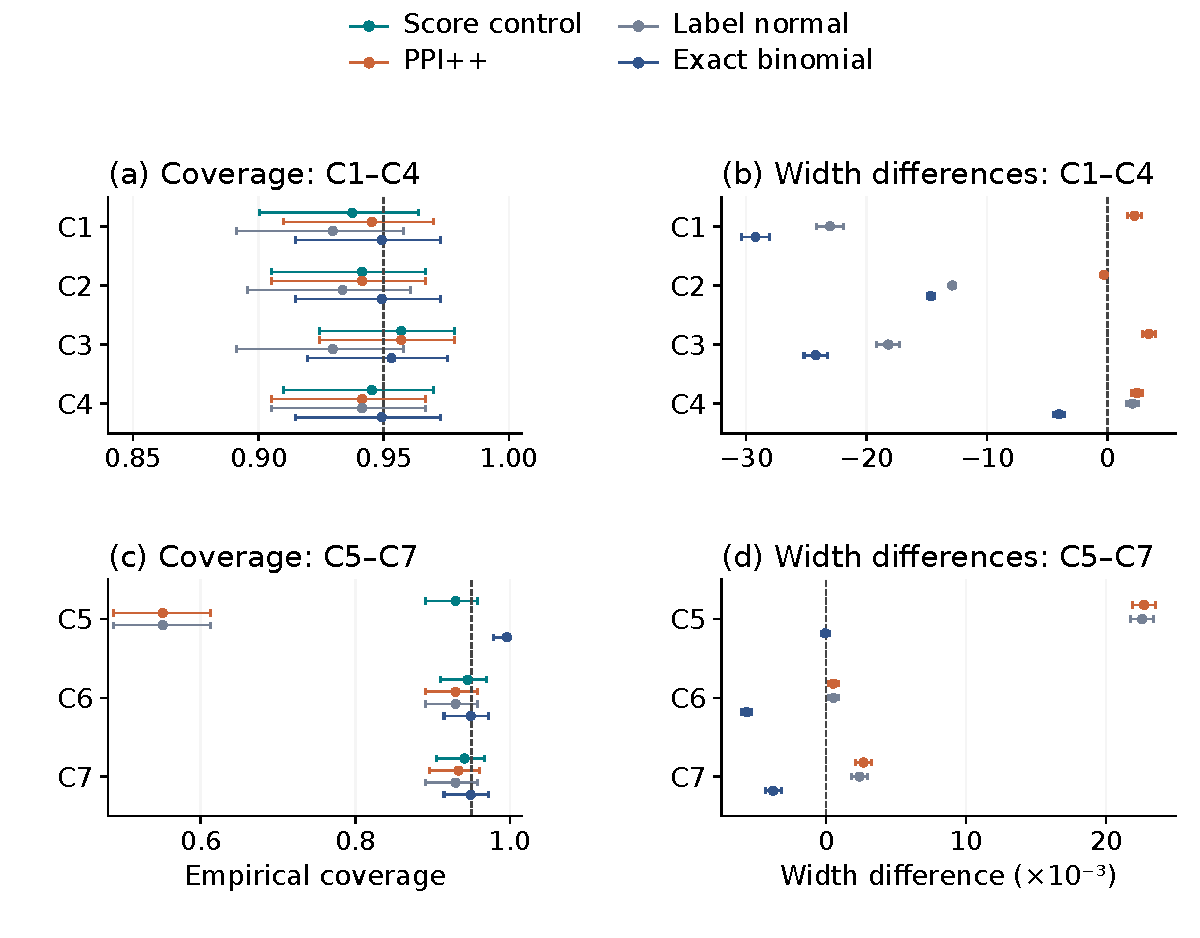
\includegraphics[width=\textwidth]{figures/coverage_width_comparison.pdf}
\caption{Coverage and paired width differences across all conditions. (a,c) Empirical coverage with pointwise 95\% exact-binomial limits; dashed lines indicate nominal coverage. (b,d) Score-control minus comparator mean widths with paired-$t$ limits; negative values mean narrower. Colors identify the comparator in width panels and the interval method in coverage panels. Coverage and width scales differ between rows. PPI is retained in the tables and Figure~\ref{fig:rare}. No interval here is multiplicity-adjusted.}
\label{fig:comparison}
% @evidence[[analysis_results.json#/cases]]
\end{figure}

\subsection{Coverage Estimates Do Not Establish Nominal Validity}
Score-control coverage ranges from $0.929688$ in C5 to $0.957031$ in C3. The pooled recorded coverage is $0.942522$, and the pooled mean width is $0.129888$. These aggregates describe the evaluated mix of conditions, not a population of application domains. They cannot replace the condition-specific comparisons, and we do not attach an independence-based binomial interval to the pooled figure.
% @evidence[[paper_data.json#/final_evaluation/metrics/coverage]]
% @evidence[[paper_data.json#/final_evaluation/metrics/mean_width]]
% @evidence[[analysis_results.json#/cases]]

All score-control pointwise coverage intervals include the nominal level. This is evidence of limited resolution, not a proof that nominal coverage holds. In particular, the interval for C5 is $[0.891151,0.957799]$, which is compatible with material undercoverage. Stabilization and the absence of collapsed intervals do not close this gap. Conversely, these finite records do not diagnose a specific adaptivity or implementation failure. Missing generator and gate diagnostics remain unknown rather than being classified as either validity failures or harmless performance losses.
% @evidence[[analysis_results.json#/cases/4/methods/candidate]]

\subsection{Low-Prevalence Failure Analysis}
C5 has recorded truth $\mu=0.0068$. Evaluated PPI++ and labeled normal intervals each cover in $0.550781$ of repetitions, with pointwise limits $[0.487609,0.612764]$. Each has 115 zero-width intervals. Score control has no zero-width intervals and coverage $0.929688$; evaluated PPI has two collapsed intervals and coverage $0.941406$. Exact-binomial coverage is $0.996094$, with limits $[0.978429,0.999901]$.
% @evidence[[analysis_results.json#/cases/4]]

Figure~\ref{fig:rare} shows the width distribution rather than only a ratio to the narrow comparator. The mass at zero and low coverage invalidate an interpretation of the PPI++ mean width as a stand-alone efficiency achievement in this condition. They do not, by themselves, identify every internal cause of a coverage miss. Boundary stabilization is a plausible source-level reason to expect fewer mechanical collapses, but the final records lack a matched stabilization ablation and a separately verified source snapshot.

The score-control and exact-binomial mean widths are $0.038898$ and $0.038945$, respectively. Their paired difference is $-0.000047$, with interval $[-0.000321,0.000227]$. Therefore, the records do not resolve a width advantage over exact inference in the condition where severe asymptotic undercoverage is most visible. The exact interval also has higher observed coverage. These observations defeat a simple ``repair collapse while becoming narrower'' interpretation.
% @evidence[[analysis_results.json#/cases/4]]

\begin{figure}[t]
\centering
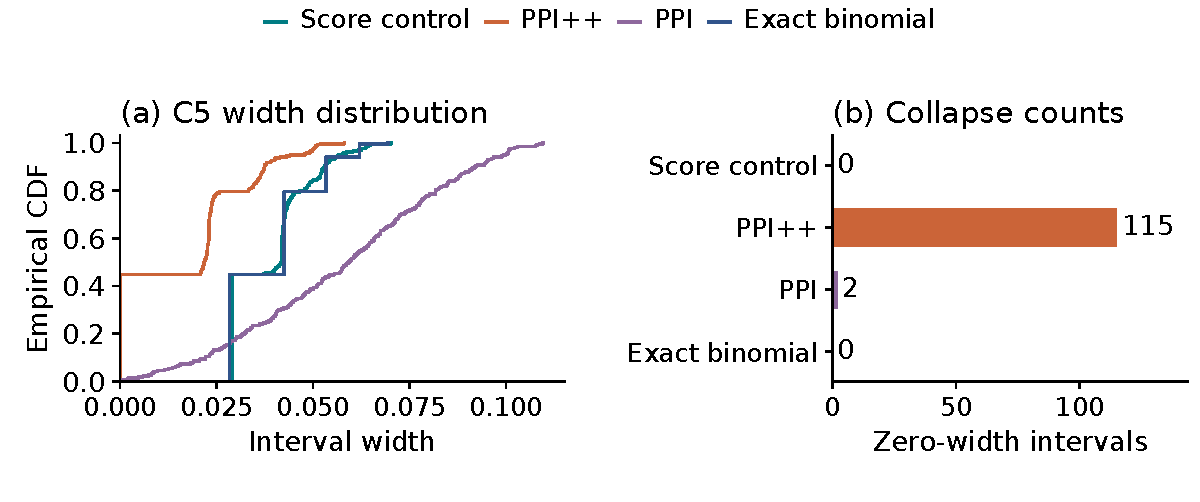
\includegraphics[width=\textwidth]{figures/rare_outcome_diagnostic.pdf}
\caption{C5 rare-outcome diagnostic, using all 256 endpoint records. (a) Empirical CDFs retain the mass at zero on a linear width axis. (b) Collapsed-interval counts. Labeled normal inference, omitted from this four-method display, also has 115 zero-width intervals. The associated coverage values appear in Table~\ref{tab:coverage}. Avoiding collapse does not establish nominal coverage or superiority to exact-binomial inference.}
\label{fig:rare}
% @evidence[[analysis_results.json#/cases/4]]
\end{figure}

\section{Discussion and Limitations}
\paragraph{A possibility result is not an empirical guarantee.}
Equation~\ref{eq:excess} identifies why frozen-score transformation can help: it can reduce the discrepancy between a control and the conditional outcome mean without modifying the predictor. But the empirical evidence shows that this opportunity need not overcome fitting noise, fold effects, and interval stabilization. Even a genuinely favorable variance calculation would not establish coverage for the returned interval. The separate bounded construction makes this distinction explicit rather than retrospectively assigning its guarantee to an asymptotic output.

\paragraph{No isolated attribution to nonlinear calibration.}
The observed method differs from its comparators in calibration, sample separation, weighting, variance estimation, and boundary handling. There is no executed matched affine-only comparison, no observed oracle frontier, and no measured safety-track interval. Consequently, the C2 result is evidence about whole evaluated configurations. It cannot establish that splines caused the gain or that cross-fitting improved width. The unavailable controlled comparisons are missing evidence, not measured negative results.

\paragraph{Sampling and source provenance restrict interpretation.}
The iid common-population assumptions are central to both correction and the safety argument. The archive does not identify whether each generator satisfies them, whether sampling masks are independent, or whether population truths were constructed analytically or from a finite external pool. We retain the stipulated population target and recorded truths, while avoiding a stronger certification of the sampling design. Likewise, source hashes preserve provenance, but readable method-family alignment does not establish byte-level identity with the sealed executable. This limits attribution without erasing the recorded endpoint comparison.

\paragraph{Reproducibility is partial, not end-to-end.}
The included extraction script reproduces the numerical tables, plotted uncertainty, and width distributions from the read-only evidence registry. It does not recreate the unknown generators or rerun the original evaluation. The source archive and seeds document what is available, but missing $n,N$, data versions, and final implementation snapshot prevent an honest claim of full experimental reproducibility. There are no measured named-dataset results, verified transfer results, or robustness analyses beyond the recorded conditions. These omissions materially limit external validity.

\paragraph{Practical interpretation.}
For fixed-input comparisons, assess coverage before interpreting width. Paired differences remain meaningful when comparator widths vanish, and exact inference supplies an important boundary reference. Selecting an interval after observing its realized width requires its own coverage argument. Here, these principles reveal a modest local gain and substantial comparator dependence, not a generally preferable interval. They motivate controlled follow-up rather than a deployment recommendation.

\section{Conclusion}
Frozen labels, unlabeled observations, and predictions do not mathematically eliminate all room for more efficient mean inference. A score-only control can exploit a better approximation to the conditional outcome mean; the fixed-control variance identity specifies this opportunity and the information it cannot recover. Whether a fitted procedure converts that opportunity into \emph{valid, narrower intervals} is a separate empirical and theoretical question.

The paired records provide a bounded answer. Score control is slightly narrower than evaluated PPI++ in C2, but wider in the other six conditions. In the low-prevalence condition it avoids observed collapsed intervals and has much higher coverage than two asymptotic comparators, yet its width advantage over exact-binomial inference is unresolved and nominal validity remains unestablished. Missing calibration ablations prevent a component-level interpretation, and missing generation metadata prevent reconstruction of the complete study. The defensible conclusion is therefore condition-specific: inference-side flexibility may change width, but this evidence does not establish a uniformly shorter, statistically valid replacement for existing intervals under fixed inputs.
% @evidence[[analysis_results.json#/cases]]

\clearpage
\bibliography{references}
\bibliographystyle{iclr2026_conference}

\clearpage
\appendix
\section{Supplementary Information}
\subsection{Complete Paired Interval Comparisons}
\label{sec:complete}
The following tables retain every evaluated inferential comparator and condition. Widths use the recorded endpoint difference; a zero-width count is an exact equality diagnostic, not an indicator that the true population mean is known. Coverage limits use equal-tailed binomial inversion across repetitions. The paired mean-difference limits use Equation~\ref{eq:paired}. No threshold-based filtering or multiplicity adjustment is applied. Uncertainty about the repetition sampling design also applies to these limits.
% @evidence[[paper_data.json#/final_evaluation/evaluation_evidence/episodes]]

\begin{longtable}{llrrr}
\caption{Complete marginal interval summaries. Limits in brackets are pointwise 95\% coverage intervals; $Z$ is the count of zero-width intervals.}\label{tab:complete}\\
\toprule
Condition & Method & Coverage [limits] & Mean width & $Z$\\
\midrule
\endfirsthead
\toprule
Condition & Method & Coverage [limits] & Mean width & $Z$\\
\midrule
\endhead
% @evidence[[paper_data.json#/final_evaluation/evaluation_evidence/episodes]]
C1 & Score control & 0.938 [0.900, 0.964] & 0.14183 & 0 \\
C1 & PPI++ & 0.945 [0.910, 0.970] & 0.13960 & 0 \\
C1 & PPI & 0.945 [0.910, 0.970] & 0.14053 & 0 \\
C1 & Label normal & 0.930 [0.891, 0.958] & 0.16486 & 0 \\
C1 & Exact binomial & 0.949 [0.915, 0.973] & 0.17104 & 0 \\
\midrule
C2 & Score control & 0.941 [0.905, 0.967] & 0.06977 & 0 \\
C2 & PPI++ & 0.941 [0.905, 0.967] & 0.07007 & 0 \\
C2 & PPI & 0.941 [0.905, 0.967] & 0.07041 & 0 \\
C2 & Label normal & 0.934 [0.896, 0.961] & 0.08266 & 0 \\
C2 & Exact binomial & 0.949 [0.915, 0.973] & 0.08442 & 0 \\
\midrule
C3 & Score control & 0.957 [0.924, 0.978] & 0.15437 & 0 \\
C3 & PPI++ & 0.957 [0.924, 0.978] & 0.15094 & 0 \\
C3 & PPI & 0.961 [0.929, 0.981] & 0.15224 & 0 \\
C3 & Label normal & 0.930 [0.891, 0.958] & 0.17257 & 0 \\
C3 & Exact binomial & 0.953 [0.920, 0.976] & 0.17859 & 0 \\
\midrule
C4 & Score control & 0.945 [0.910, 0.970] & 0.17167 & 0 \\
C4 & PPI++ & 0.941 [0.905, 0.967] & 0.16922 & 0 \\
C4 & PPI & 0.965 [0.934, 0.984] & 0.19605 & 0 \\
C4 & Label normal & 0.941 [0.905, 0.967] & 0.16962 & 0 \\
C4 & Exact binomial & 0.949 [0.915, 0.973] & 0.17570 & 0 \\
\midrule
C5 & Score control & 0.930 [0.891, 0.958] & 0.03890 & 0 \\
C5 & PPI++ & 0.551 [0.488, 0.613] & 0.01620 & 115 \\
C5 & PPI & 0.941 [0.905, 0.967] & 0.05742 & 2 \\
C5 & Label normal & 0.551 [0.488, 0.613] & 0.01633 & 115 \\
C5 & Exact binomial & 0.996 [0.978, 1.000] & 0.03894 & 0 \\
\midrule
C6 & Score control & 0.945 [0.910, 0.970] & 0.16540 & 0 \\
C6 & PPI++ & 0.930 [0.891, 0.958] & 0.16486 & 0 \\
C6 & PPI & 0.930 [0.891, 0.958] & 0.16486 & 0 \\
C6 & Label normal & 0.930 [0.891, 0.958] & 0.16486 & 0 \\
C6 & Exact binomial & 0.949 [0.915, 0.973] & 0.17104 & 0 \\
\midrule
C7 & Score control & 0.941 [0.905, 0.967] & 0.16727 & 0 \\
C7 & PPI++ & 0.934 [0.896, 0.961] & 0.16459 & 0 \\
C7 & PPI & 0.988 [0.966, 0.998] & 0.19287 & 0 \\
C7 & Label normal & 0.930 [0.891, 0.958] & 0.16486 & 0 \\
C7 & Exact binomial & 0.949 [0.915, 0.973] & 0.17104 & 0 \\
\midrule
\bottomrule
\end{longtable}

\begin{longtable}{llrr}
\caption{Paired score-control minus comparator width differences. Negative values indicate narrower recorded intervals, not a coverage-adjusted advantage.}\label{tab:paired}\\
\toprule
Condition & Comparator & Mean difference & Pointwise 95\% limits\\
\midrule
\endfirsthead
\toprule
Condition & Comparator & Mean difference & Pointwise 95\% limits\\
\midrule
\endhead
% @evidence[[paper_data.json#/final_evaluation/evaluation_evidence/episodes]]
C1 & PPI++ & +0.002231 & [+0.001631, +0.002831] \\
C1 & PPI & +0.001302 & [+0.000690, +0.001913] \\
C1 & Label normal & -0.023034 & [-0.024169, -0.021900] \\
C1 & Exact binomial & -0.029209 & [-0.030341, -0.028077] \\
\midrule
C2 & PPI++ & -0.000302 & [-0.000400, -0.000203] \\
C2 & PPI & -0.000644 & [-0.000742, -0.000547] \\
C2 & Label normal & -0.012893 & [-0.013143, -0.012644] \\
C2 & Exact binomial & -0.014651 & [-0.014900, -0.014401] \\
\midrule
C3 & PPI++ & +0.003429 & [+0.002896, +0.003962] \\
C3 & PPI & +0.002130 & [+0.001550, +0.002710] \\
C3 & Label normal & -0.018195 & [-0.019163, -0.017227] \\
C3 & Exact binomial & -0.024218 & [-0.025186, -0.023250] \\
\midrule
C4 & PPI++ & +0.002452 & [+0.001972, +0.002933] \\
C4 & PPI & -0.024381 & [-0.025514, -0.023247] \\
C4 & Label normal & +0.002056 & [+0.001575, +0.002537] \\
C4 & Exact binomial & -0.004025 & [-0.004505, -0.003544] \\
\midrule
C5 & PPI++ & +0.022702 & [+0.021895, +0.023508] \\
C5 & PPI & -0.018525 & [-0.021644, -0.015407] \\
C5 & Label normal & +0.022565 & [+0.021741, +0.023389] \\
C5 & Exact binomial & -0.000047 & [-0.000321, +0.000227] \\
\midrule
C6 & PPI++ & +0.000537 & [+0.000179, +0.000894] \\
C6 & PPI & +0.000537 & [+0.000179, +0.000894] \\
C6 & Label normal & +0.000537 & [+0.000179, +0.000894] \\
C6 & Exact binomial & -0.005638 & [-0.005995, -0.005281] \\
\midrule
C7 & PPI++ & +0.002681 & [+0.002112, +0.003251] \\
C7 & PPI & -0.025593 & [-0.026689, -0.024498] \\
C7 & Label normal & +0.002409 & [+0.001840, +0.002978] \\
C7 & Exact binomial & -0.003766 & [-0.004334, -0.003197] \\
\midrule
\bottomrule
\end{longtable}

The full-range interval is $[0,1]$ in the records and covers the recorded binary-mean truths. It is a check on the endpoint/target convention, not a competitive width baseline. Raw width ratios can be dominated by zero or near-zero denominators in C5. We therefore do not interpret the retained pooled ratio as a multiplicative efficiency advantage, and do not infer how any denominator regularization was implemented.
% @evidence[[paper_data.json#/final_evaluation/evaluation_evidence/episodes]]
% @evidence[[paper_data.json#/final_evaluation/metrics/width_ratio_ppiplus]]

\subsection{Calibration and Interval Implementation}
\label{sec:implementation}
Readable source copies are supplied under \path{source_evidence/calibration/}. The entrypoint specification declares \path{program.py}; the functions below describe that archive. The final evaluation's recorded source-tree hash is not independently reconstructed from these copies. Thus, these locations substantiate source-level choices, not a stronger assertion that every sealed endpoint came from an identical file tree.

\paragraph{Training-only model choice.}
The basis contains the raw score and positive-part hinges $(S-\kappa)_+$. The training outcome mean supplies the intercept. Each feature is centered and scaled on the training fold; standard deviations are floored at $10^{-8}$. For a training count $m$, a penalty $\lambda$ solves
\begin{equation}
\widehat\beta_\lambda=(Z^\top Z/m+\lambda I)^{-1}Z^\top(Y-\overline Y)/m.
\end{equation}
The effective degrees of freedom are $d=1+\operatorname{tr}\{(Z^\top Z/m+\lambda I)^{-1}Z^\top Z/m\}$. The GCV denominator is $\max(1-d/m,1/m)^2$. This score selects among the available basis/penalty pairs and the constant fit \citep{HoerlKennard1970,Golub1979GCV}. The smallest training size for nonconstant fitting is four; score range below $10^{-12}$ keeps the intercept. None of these thresholds is a measured tuning optimum.
% @evidence[[source_evidence/calibration/program.py#L58-L93]]

\paragraph{Randomization and output.}
The reset seed initializes the local random generator used for permutations. State is cleared between repetitions; labels are not pooled across them. Only the predefined outcome and score arrays enter inference. The interface reports an estimate and bounded endpoints, not calibration diagnostics. In the exact small-$n$ branch, beta quantiles implement equal-tailed binomial inversion. Otherwise the reported point estimate is the clipped corrected mean, while the interval center is $c$ from Equation~\ref{eq:stabilized}. These need not be identical. The stabilization is not an exact Wilson interval, even though its algebra resembles score-based boundary adjustments \citep{Newcombe1998,AgrestiCoull1998}.
% @evidence[[source_evidence/calibration/program.py#L195-L259]]

\paragraph{Unmeasured functions.}
The archive exposes \texttt{fit\_affine\_calibrator} and an internal affine option with the same clipping and penalty grid but no hinges. The reporting helper also defines an oracle variance calculation. Neither function supplies an executed controlled comparison in the sealed evidence. The preparation note's statement that experiments had not yet been run describes preparation time; it does not negate the subsequently supplied endpoint records. Conversely, later records do not supply missing affine or bounded-track results.
% @evidence[[source_evidence/calibration/program.py#L188-L192]]
% @evidence[[source_evidence/calibration/study.py#L12-L26]]

\subsection{Fixed-Control Variance and Separate Safety Argument}
\label{sec:theory}
\paragraph{Variance decomposition.}
Assume the iid sampling model from the main text, $n,N$ fixed, and a fixed square-integrable $g$. Write $Y=m(S)+\varepsilon$, where $\E[\varepsilon\mid S]=0$. Independence between the labeled and unlabeled samples gives Equation~\ref{eq:fixed}. Let $h=g-m$. Orthogonality of $\varepsilon$ and score functions yields
\begin{align}
\Var(Y-\rho g)&=\E[\Var(Y\mid S)]+\Var\{(1-\rho)m-\rho h\},\\
\Var(g)&=\Var(m+h).
\end{align}
The cross term cancels because $(1-\rho)/n=\rho/N$. The remaining coefficients are
\begin{equation}
\frac{(1-\rho)^2}{n}+\frac{\rho^2}{N}=\frac{1}{n+N},\qquad
\rho^2\left(\frac1n+\frac1N\right)=\frac{\rho}{n}.
\end{equation}
This proves Equations~\ref{eq:oracle}--\ref{eq:excess}. Additive constants in $g$ cancel from the estimator, consistent with the variance rather than uncentered squared-error excess. If $\Pi_{\mathrm{aff}}m$ is the $L^2$ projection onto unrestricted affine functions of $S$, including an intercept, the oracle reduction relative to the best such affine control is
\begin{equation}
\frac{N}{n(n+N)}\E\bigl[(m-\Pi_{\mathrm{aff}}m)^2\bigr].
\end{equation}
The projection residual has mean zero. Constant scores reduce the affine space to constants. This calculation concerns unrestricted population controls; the clipped, regularized fitted affine family is not that same class. No recorded condition is shown to attain this reduction.
% @evidence[[source_evidence/calibration/METHOD.md#Oracle-frontier-and-asymptotic-qualifications]]
% @evidence[[source_evidence/calibration/study.py#L12-L26]]

\paragraph{Why fitted-control inference requires more.}
For fixed $g$, elementary variance algebra suffices. For estimated $g_{-k}$, conditional sample separation preserves the correction's expectation under the iid model, but unconditional covariances across folds remain. First-order inference requires additional control of fitted-function error and variance estimation, as emphasized more generally in semiparametric theory \citep{Robinson1988,VanDerVaart1998,Chernozhukov2018DML}. The archive does not establish the required rates for its finite dictionary/GCV rule in each condition. The Efron--Stein perspective also emphasizes accounting for estimator sensitivity rather than treating fitted components as fixed \citep{EfronStein1981}. We use no such inequality to certify the returned interval.

\paragraph{Bounded safety construction.}
For a held-out component sample $A_1,\ldots,A_m$ with known range length $B$, the archived radius is
\begin{equation}
b(A,\delta)=\min\left\{B,\sqrt{\frac{2s_A^2\log(4/\delta)}{m}}
+\frac{7B\log(4/\delta)}{3(m-1)}\right\},\qquad m\geq2.
\label{eq:eb}
\end{equation}
For a singleton, it uses $B$. This is a conservative two-sided empirical-Bernstein form \citep{MaurerPontil2009}; known boundedness, as in classical concentration arguments \citep{Hoeffding1963}, is essential. Capping at $B$ cannot invalidate a bound because both the sample and population means lie in the support interval. The variance-sensitive term can be useful, but the additive range term can make the interval substantially wider than an asymptotic one. Related variance-aware bounds are studied in other settings \citep{Audibert2009}; those sequential results are not empirical evidence here.
% @evidence[[source_evidence/calibration/program.py#L109-L119]]

For $K=2$ folds, each residual mean and each unlabeled control mean receives error probability $\delta=\alpha/(2K)$. Conditional on the opposite labeled training sample, the residuals have support $[-\rho,1]$ and the unlabeled controls have support $[0,\rho]$. Their expectations sum to $\mu$. A union bound across the $2K$ component events therefore controls the probability of any failure by $\alpha$, without requiring independence across the fitted folds. On this joint event, each fold interval contains $\mu$; averaging lower and upper endpoints using fixed nonnegative weights summing to one preserves containment. Intersecting with $[0,1]$ preserves containment of a binary mean. The implementation replaces an empty numerical intersection by the full range.
% @evidence[[source_evidence/calibration/program.py#L129-L185]]

This is a coverage argument for the separate construction under the stated sampling and support assumptions. It is not an empirical coverage estimate, a width comparison, or a theorem for Equation~\ref{eq:stabilized}. No width-dependent choice between the two constructions is justified by the union bound as implemented.

\subsection{Evidence Extraction and Reproducibility Boundaries}
\label{sec:reproduce}
\paragraph{Inputs and deterministic outputs.}
The read-only \path{paper_data.json} is the primary numerical input. The script \path{scripts/build_artifacts.py} reads the final endpoint records, checks paired differences against the supplied summaries, and writes \path{analysis_results.json}, the tables under \path{tables/}, and both quantitative figure groups under \path{figures/}. Each quantitative figure is exported as vector PDF and 300-DPI PNG, with an adjacent provenance sidecar recording its inputs. The overview figure is separately prepared from the method description and is not a quantitative result plot.
% @evidence[[scripts/build_artifacts.py]]

The recorded repetition seeds are 1001--1256. Truths are $0.353333\ldots$ in C1, C2, C6, and C7; $0.5$ in C3; $0.41$ in C4; and $0.0068$ in C5. These are record values, not recovered generation parameters. No condition-specific sample sizes, datasets, data licenses, or original data-download instructions can be reconstructed from the staged evidence. An end-to-end runner would require these missing inputs; the archived \path{study.py} is a collection of reporting helpers, not such a runner.
% @evidence[[analysis_results.json#/seeds]]
% @evidence[[analysis_results.json#/cases]]
% @evidence[[source_evidence/calibration/study.py]]

\paragraph{Uncertainty choices and unperformed analyses.}
The paired-$t$ limits describe repeated width differences under their usual sampling approximation. We did not run a bootstrap, a jackknife, a sensitivity sweep, or a new evaluation. Bootstrap references describe alternative distribution-estimation tools \citep{Efron1979,EfronTibshirani1993}, not analyses performed for this paper. Recomputing interval summaries from archived records cannot repair an unknown sampling mechanism. The included source manifest records local file hashes and distinguishes them from the final evaluator's source-tree identifiers.

\paragraph{Environment and commands.}
The reproduction guide records the exact paper-analysis package versions, a CPU-only command for regenerating the tables and plots, and the validation commands. These are the environment versions used for manuscript extraction, not recovered versions of the sealed evaluation environment. No evaluation runtime is inferred from the plot-generation runtime. No prohibited literature was intentionally searched or consulted: citation remediation used exact permitted starter works and pre-screened historical foundations, without citation-network traversal. Rejected DOI/title mismatches are recorded as retrieval errors, not used as references.

\paragraph{Qualification and auditing.}
The independently read final record reports a completed evaluation and a qualified outcome. Its retained endpoint measurements remain the scientific evidence. The acceptance outcome is not interpreted as a guarantee of validity, superiority, or successful source verification. Candidate diagnostics remain unverified; gate-specific causes not supplied in the evidence are unknown. The claim map separately records qualification sources, endpoint sources, readable implementation locations, and literature provenance.
% @evidence[[paper_data.json#/final_evaluation/status]]
% @evidence[[paper_data.json#/final_evaluation/outcome]]
% @evidence[[paper_data.json#/final_evaluation/evaluation_evidence/candidate_diagnostics_trust]]

\subsection{LLM Usage}
LLM-based assistance was used for research-direction proposals, preparation of candidate implementations, reference-query planning, manuscript framing and drafting, deterministic analysis-script construction, and evidence/format checks. The supplied evaluation records, not LLM estimates, provide the empirical observations. No additional scientific evaluation was performed during manuscript preparation. Automated source inspection and claim checks are not independent statistical verification. No claim of human review or manual experimental replication is made. The manuscript's limitations, including missing controlled comparisons and generation metadata, are retained rather than filled with inferred results.

\end{document}
